\documentclass[12pt, french]{report}

%%%%%%%%%% Packages externes utilisés %%%%%%%%%%%%%%%%%%%
\usepackage[french]{babel}
\selectlanguage{french}
\usepackage[T1]{fontenc}
\usepackage[utf8]{inputenc}
\usepackage{textcomp}
\usepackage{macro}
\usepackage{eso-pic,graphicx,transparent}
\usepackage{hyperref}
\usepackage{afterpage}
\usepackage{xcolor}
\usepackage[demo]{graphicx}
\usepackage{subfig}
\usepackage{amsmath, amsthm, amssymb, amsfonts}
%La mise en page du rapport, NE PAS MODIFIER.
\usepackage{geometry}
\geometry{
   a4paper,
   left=20mm,
   right=20mm,
   top=20mm,
   bottom=20mm
}

\begin{document}
\begin{titlepage}

\begin{center}

\AddToShipoutPicture*{\BackgroundPic}

{\large Master 1 Informatique et Ingénierie des Systèmes Complexes (IISC)}\\[0.5cm]

{\large \textbf{Université de Cergy-Pontoise}}\\[1.5cm]

{\large \textbf{Projet de synthèse}}\\[0.5cm]

% Title
\rule{\linewidth}{0.5mm} \\[0.4cm]
{ 
    \huge \bfseries Résolution de labyrinthes par véhicule intelligent \\[0.5cm]
    \huge Micromouse\\[0.4cm]
}
\rule{\linewidth}{0.5mm} \\[0.5cm]

\begin{center}
\begin{minipage}{0.5\textwidth}
   \large
    \emph{rapporteur :}

\end{minipage}%
\end{center}

\vspace{5mm}
% Author and supervisor
\noindent
\begin{minipage}{0.5\textwidth}
  \begin{flushleft} \large
    \emph{Auteurs :}\\
    Djahid \textsc{ABDELMOUMENE}\\
    Amine \textsc{AGRANE}\\
    Ishak \textsc{AYAD}\\
    Donald \textsc{LAY}
  \end{flushleft}
\end{minipage}%
\begin{minipage}{0.5\textwidth}
  \begin{flushright} \large
    \emph{Tuteur technique :} \\
    Pr.~Alexandre \textsc{PITTI}\\
    \emph{Encadrant de gestion de projet :}
    Pr.~Tianxiao \textsc{LIU}
  \end{flushright}
\end{minipage}

\noreffig{pics/MMLogo.pdf}{12.82cm}{8.2cm} \\

\vspace*{\fill}
% Bottom of the page
{\large Rendu le\\ \today}

\end{center}
\end{titlepage}

\clearpage

\thispagestyle{empty}
\section*{Remerciements}

\clearpage
\thispagestyle{empty}
\section*{Résumé et abstract}
\subsection*{Résumé}

\subsection*{Abstract}

\clearpage
\setcounter{page}{1}
\tableofcontents
\listoffigures

\clearpage

\chapter{Introduction}
\paragraph{Chapeau du chapitre}
\section{Contexte du projet}
\label{sec:introduction_contexte_du_projet}

\paragraph{Chapeau}
\paragraph{
ère des machines autonomes
\\ce qui existe : pilotage automatique en voies rapides
\\autre domaine d'application :
\\médical
\\secourisme
\\jeux vidéos
\\
}

\section{Objectifs du projet}
\label{sec:introduction_objectifs_du_projet}

\paragraph{Chapeau}
\paragraph{
< EQUIPE >
\\ IHM <date>
\\ Interface de simulation <date>
\\ Conception unitaire d'un prototype <date>
\\ Environnement physique <date>
\\ Scénario multi-souris évoluant dans l'environnement physique élaboré avec une IA additionnelle (les micromouses se confrontent alors mutuellement ou par équipe dans un jeu (à décider). <date>
}

\section{Mise en scénario}
\label{sec:introduction_mise_en_scenario}

\paragraph{Chapeau}
\paragraph{
I - Simulation
\\ -> Simulation d'un environnement physique
\\ -> Moyen visuel de rendre compte de l'avancement du processus d'apprentissage de la micromouse (à reformuler) sur l'IHM. Le visuel (IHM) doit se rapprocher de celui affiché sur l'interface de simulation (environnement simulé)
\\ -> Constater des mouvements physique en temps réél en adéquation avec les informations de simulation (à plat le sol ou surélevé)
\\II - Mise en route de la micromouse dans l'environnement physique.
\\ -> premier départ : apprentissage/mapping du labyrinthe
\\ -> second départ : vers l'arrivée par le biais du chemin le plus court (A*)
\\ III - Scénario multi-mouse
\\ < JEU A DEFINIR >
}

\section{Organisation du rapport}
\label{sec:introduction_organisation_du_rapport}

\paragraph{
Cahier des charges (bla bla + permettant de mettre en évidences les contraintes techniques suivantes : ... ) -> Parties techniques -> Rendu final -> Gestion de projet -> Conclusion.
}
\clearpage

\chapter{Présentation et spécification du projet}
Ce chapitre présente le cahier des charges (CDC) du projet et les
spécifications techniques, il contient les principaux éléments nécessaires
pour comprendre le positionnement marketing du futur produit et la
conception technique. Il mentionne également des informations relatives au
développement du produit dans sa globalité et son architecture.

\section{Étude du marché} \label{sec:etudeMarche}
Une compétition Micromouse est un évènement durant lequel plusieurs équipes
s'affrontent en opposant leurs robot souris, l'objectif étant de résoudre un
labyrinthe le plus rapidement possible.  Ces compétitions sont organisées
depuis la fin des années 1970 et ont lieu un peu partout autour du monde.

\paragraph{Historique et Origine}
Le magazine "IEE Spectrum magazine" est à l'origine de l'apparition des
compétitions Micromouse. C'est un magazine anglophone qui vise à couvrir les
tendances et avancés majeures dans les domaine des technologies, de
l'ingénierie et des sciences. En 1977, le magazine mets au défi ses lecteurs en
leur proposant de concevoir et construire un robot "micromouse" pouvant
résoudre un labyrinthe. Le robot devait agir selon sa propre logique et
résoudre un labyrinthe imaginé par les rédacteurs du magazine IEE Spectrum.
Cette compétition fut appelée ‘The Amazing Micromouse Competition’. Elle pris
place à New York lors de la conférence nationale sur l'informatique en 1979.
Cet évènement couvert pas de grands médias tels que les chaines CBS et ABC
ainsi que la journal The New York Times.  Le grand succès de cette première
édition ainsi que sa large médiatisation participa au gain de popularité des
compétions Micromouse pour les années à venir.  En quelques années, le défi des
micromouse était devenu un événement mondial. En 1980, le premier concours
européen a eu lieu à Londres, suivi un an plus tard par un une compétition
organisée à Paris. Le Japon a annoncé l'organisation du premier tournoi mondial
de Micromouse qui aura lieu à Tsubaka en Août 1985. La même année, l'IEE
(devenue l'Institution of Engineering and Technology) a organisé un concours
international à Londres.  Au début des année 1990 des clubs Micromouse ont
commencé à faire leurs apparition au seins des écoles et universités. La "IEE
Micromouse Competition" bénéficie au jours d'aujourd'hui d'une grande
popularité auprès des étudiants du domaine informatique ou électronique.
\newpage
    
\fig{pics/old_micromouse.jpg}{16cm}{12cm}
{Ancienne génération de Micromouse (Pacific Northwest National Laborator, 1980)}{mmcomp}

\paragraph{Organistaions des compétitions}
   Au vu du nombre importants de compétition Micromouse ayant lieu chaque année,
certaines règles et conditions peuvent varier d'une compétition à l'autre.
Néanmoins, ils existent des éléments généralement communs à toutes les
compétitions : 
\\ 

\begin{itemize}

\item
   Le labyrinthe standard de micromouse mesure environ $2.5m^2$
et consiste en une grille de cellules (matrice) de 16 sur 16. Chaque micromouse
est autorisée à effectuer un certain nombre de recherches afin de déterminer le
chemin le plus court vers l'objectif.  La micromouse devra garder une trace de
sa position, découvrir les murs en explorant le labyrinthe et détectez quand
elle a atteint son l'objectif (sortie du labyrinthe). \\

\item
   La notation est basée à la fois sur la course la plus rapide et sur le temps
total consommé pour toutes les courses. Les concurrents n'ont pas le droit de
communiquer avec leurs micromouse.  Il existe de nombreuses versions de règles
selon la compétition, et il existe un certain nombre de variations mineures sur
la façon dont la le score de la souris est déterminé. \\

\end{itemize}


\clearpage
\section{Fonctionnalités attendues} \label{sec:foncAttendues}
\paragraph{
   Dans la section [\ref{sec:miseEnScenario}] le lecteur peut observer que le
produit proposé fournit plusieurs options ie:fonctionnalités pour tester et
manipuler différentes entités dans les deux environnements, physique et
simulé dans cette section nous allons introduire ces fonctionnalités et
expliquer les cas d'utilisation de ces derniers.}

\subsection{Vue d’ensemble du système} \label{sec:vueEns}

\vspace{5mm}
Le produit permet à l'utilisateur de simuler un véhicule autonome se déplaçant 
dans un labyrinthe et en essayant de trancher le point d'arriver, le labyrinthe 
est créé soit manuellement ou en insérant un fichier de configuration, ainsi la 
simulation pourra se lancer et l'utilisateur pourra observer le déplacement de 
la micro mouse et en même temps d'observer le journal et les statistiques de la 
simulation qui sont modifiées et stockées au fur et à mesure de la simulation, 
ainsi que les valeurs des différents composants de l'engin. \\

En outre, l'utilisateur du produit peut modifier le labyrinthe réel et d'y mettre 
le véhicule dedans pour lancer une observation physique, ainsi qu'il pourra voir 
sur sa machine sur un autre logiciel de visualisation le déplacement et les valeurs 
retournées par l'engin. \\

Le schéma suivant illustre le diagramme de cas d'utilisation du produit.


\fig{pics/UC_micromouse.png}{20cm}{12.5cm}
{Le diagramme de cas d'utilisation du système}{UCMicromouse}

\subsection{Services fournis par le produit} \label{sec:serLogiciel}

\paragraph{Simulation :}La simulation offre à l'utilisateur une diversité de choix 
et d'API comme la création du labyrinthe soit avec un fichier de configuration ou 
manuellement et le choix de la complexité de l'algorithme de recherche du plus court chemin, 
en outre l'utilisateur peut visualiser le journal de la simulation et les statistiques 
sur la partie information sur la simulation, finalement l'utilisateur pourra observer 
les valeurs des différents composants de la micro mouse.


\fig{pics/SimGUI.pdf}{17cm}{10cm}{Interface homme-machine pour la simulation}{ihmSim}

\paragraph{Véhicule réel :}


\newpage
\subsection{Fonctionnalités supplémentaires} \label{sec:foncSupplementaires}

\paragraph{Visualisation en temps réel :}La visualisation des résultats au fur et à mesure 
du temps, au moment du lancement du système l'utilisateur peut lancer un logiciel, c'est le 
logiciel de visualisation des résultats de l'expérience, il permet à l'utilisateur de visualiser 
la vue du véhicule et les valeurs des capteurs au fur et à mesure de l'exploration, aussi de 
visualiser le journal de la simulation et les statistiques.

\fig{pics/visLogiciel.png}{15cm}{6cm}
{Maquette du logiciel de visualisation}{visLogiciel}

\paragraph{Multi-véhicule :} Un mini-jeu est mis en place pour les 
deux univers, simulé et réel permettant d'introduire la notion de communication 
entre différents véhicules, le jeu consiste à parcourir toutes les cases du 
labyrinthe et à la fin se situer dans la case d'arriver par un véhicule autonome 
intelligent en évitant les autres véhicules gradient communiquant entre eux. 
Ceci en utilisant les modules déjà abordés tels que la simulation et l'univers réel.

\fig{pics/GamePacman.pdf}{14cm}{7cm}
{Pac-Man avec l'entité micro mouse (Pac-Micro)}{pacMicro}

La figure [\ref{fig:pacMicro}] représente une illustration du mini-jeu, les trois chats représentent 
les gardiens du labyrinthe et le carré noir représente le véhicule intelligent qui 
doit résoudre le labyrinthe en parcourant toutes les cases tous en évitant de croiser un gradient.


\section{Conception globale du projet} \label{sec:conception}
\paragraph{
   après avoir illustré les différentes fonctionnalités du système sur la
section [\ref{sec:foncAttendues}], il va falloir expliquer plus en détails
la conception de ces fonctionnalités, en séparent la vue pour l'utilisateur
on masquera les détails techniques informatiques et on illustrera seulement
les composants ou modules fonctionnels, de l'architecturer technique et
logiciel on va présenter les différentes parties techniques nécessaires
permettant de réaliser les fonctionnalités décrites dans la section
précédente [\ref{sec:foncAttendues}]}

\subsection{Vue pour l’utilisateur} \label{sec:vueUtil}
   
   Le système offre à l'utilisateur deux choix pour l'exploiter: \\
\begin{enumerate}

   \item Le système réalisé permet à l'utilisateur d'observer le fonctionnement
 et l'évolution de la micro mouse ie:véhicule autonome dans sans monde un 
 labyrinthe de 12x12 case dans un monde physique, pour but de résoudre ce 
 labyrinthe et trouver le plus court chemin du point de départ au point final; \\

\begin{itemize}
      \item \textbf{Le labyrinthe} \\

      \item \textbf{La micro mouse} \\
\end{itemize}

   \item Le système permet aussi de simuler les fonctionnalités physiques 
dans un monde simulé, un labyrinthe de taille variante et des chemins à 
définir par l'utilisateur, aussi on peut charger un fichier de configuration 
pour créer le labyrinthe; \\

\begin{itemize}
      \item \textbf{Le labyrinthe} \\

      \item \textbf{La micro mouse} \\
\end{itemize}

   \item Finalement, l'utilisateur peut observer en temps réel l'évolution 
de la micro mouse dans son univers, cette partie permet aussi d'afficher 
les valeurs des différents composants du véhicule comme les capteurs infrarouges 
et l'accéléromètre ainsi que d'autres informations sur la simulation. \\

\begin{itemize}
   \item \textbf{Le labyrinthe} \\

   \item \textbf{La micro mouse} \\
\end{itemize}

\end{enumerate}

\subsection{Architecture technique} \label{sec:archTechnique}

   la micromouse sera composée de nombreuses parties electronique qui vont lui
permettent de fonctionner. \\


   Le plus important d'entre eux est le \textbf{PCB} (Printed Circuit Board)
qui est le corps où tous les autres composants seront soudés, il sert aussi
à les interconnecter et  leur faire communiquer. Pour cela, nous avons
trouvé un design open source \cite{Bulebule:1} conçu pour les micro-souris
qui contient tous les modules nécessaires pour notre produit final. \\


\fig{pics/PCBparts.pdf}{14cm}{10cm}{digramme de composantes dans le PCB}{pcb}


   Le cerveau de notre véhicule sera un micro contrôleur \textbf{STM32F103}
\cite{Bluepill:1} également connu sous le nom de Blue Pill, il a 64KB/128KB de
mémoire flash et 20KB de RAM fonctionnant à 72MHz. \\


   On passe ensuite aux capteurs, qui sont les composants utilisés pour
recevoir les informations du monde extérieur, qui est dans ce cas le
labyrinthe. \\


   Il y a trois types que nous allons utiliser, le premier est le
\textbf{gyroscope} qui est employé pour détecter le changement de direction
et l'angle de rotation, c'est important pour bien tracer le labyrinthe
puisque le véhicule devra faire beaucoup de manœuvres dans le labyrinthe. \\


   Ensuite, il y a \textbf{l'accéléromètre} qui, comme son nom l'indique,
détecte l'accélération, et avec le gyroscope il peut trouver la position ou
plutôt les changements de position, de micromouse, ce capteur alors sera le
seul moyen de localisation pour notre véhicule.\\


   Ces deux capteurs précédents sont généralement regroupés sur une seule
circuit électronique parce qu'ils sont sovent utilisés ensemble et ont des
fonctionnalités similaires, cela nous économise également de la place sur le
PCB. \\


   Enfin, il y a les \textbf{capteurs infrarouge} que nous utiliserons pour
obtenir la distance du véhicule des murs et autres obstacles, ils seront
placés sur toutes les directions pour évaluer plus précisément les alentours
et avoir une meilleure cartographie du labyrinthe. \\


   Nous disposerons également d'un \textbf{module bluetooth}, l'outil de
communication principal.  Lequel est utilisé pour envoyer des données en
direct à l'interface afin de déboguer et de visualiser le processus de
Mapping, ainsi que pour communiquer avec le simulateur de labyrinthe pour
recevoir les signaux des capteurs artificiels. \\


   Le contrôle du véhicule se fera avec deux \textbf{moteurs falhaber}
\cite{faulhaber:1} des deux côtés du véhicule. Les roues et leurs essieux sont
imprimés en 3d pour s'adapter au design du circuit. Aucun volant ne sera
utilisé à cause du poids supplémentaire qu'ils apportent et aussi parce que
les deux que nous avons déjà peuvent faire des manœuvres très précises avec un
code conducteur minimal. \\


   Il existe d'autres petits composants électriques ou \textbf{SMD}s (Surface
Mount Devices) tels que les résistances, condensateurs, interrupteurs,
diodes, LEDs etc... qui sont utilisés pour contrôler le courant électrique
sur le PCB.

\subsection{Architecture logicielle} \label{sec:vueLogicielle}



\section{Problématiques identifiées et solutions envisagées} \label{sec:problemesSolutions}

\paragraph{
   D'un coup d'œil, plusieurs problèmes majeurs se posent d'un point de vue
technique du projet.  Dans cette section, nous décrivons ces problèmes et
les solutions que nous y apportons.}



\subsection{Mappage et navigation} \label{sec:rechChem} 

   Pour notre véhicule, les seules données qu'il reçoit du monde extérieur sont
celles des capteurs, ce sont des signaux en temps réel des changements de
rotation et d'accélération, ainsi que les distances des murs qui sont les
principales informations que nous allons utiliser pour le traçage de la mappe. \\

   Pour transformer ces signaux en une carte 2D du labyrinthe, nous allons devoir
commencer par déterminer la position et la direction du véhicule. Pour cela,
nous utiliserons les informations du gyroscope afin de garder une copie de la
position et de la direction et de les actualiser a chaque iteration en
utilisant les données reçues. \\

   Après avoir obtenu ces entrées, nous allons les utiliser avec les informations
restantes des capteurs infrarouges pour faire la mappage proprement dite, nous
pouvons utiliser un algorithme de Flood fill pour déterminer la géométrie des
murs et/ou des obstacles. Après un peu de nettoyage et interpolation nous
devrions avoir une carte finale du labyrinthe. \\

   Une fois le tour de mapping est terminé, nous devrons trouver le chemin le plus
court entre la position du véhicule et le point d'arrivée. Une solution qui
vient à l'espritest l'algorithme A* qu'il est souvent utilisé dans les
labyrinthes et qui estalors idéale pour notre projet. Bien sûr, l'algorithme
doit être modifié pourtenir compte des erreurs occasionnelles de contrôle qui
surviennent à cause des irrégularités du monde physique.

\subsection{Contrôle du véhicule} \label{sec:ctrlComm}

Notre véhicule se compose de deux moteurs que nous devrons contrôler pour
parcourir les chemins avec fluidité, il devra faire des virages et éviter les
collisions avec les murs et autres obstacles, tout en suivant le chemin créé
pour lui. \\

Pour résoudre ces problèmes, nous allons utiliser la logique floue qui servira
à générer des signaux pour les puissances des moteurs en temps réel. La façon
dont cela fonctionne est que nous créons un moteur d'inférence et lui
fournissons des règles qui décrivent la façon dont la véhicule doit se comporter 
en se déplaçant, et le moteur utilisera ces règles ainsi que les données du
capteurs pour générer les signaux de sortie des moteurs qui seront sa décision
finale.

\subsection{Communication} \label{sec:mapMaze}
Un problème qui se pose à cause des besoins de certaines fonctionnalités du
projet est la communication, que ce soit pour déboguer et visualiser les
données du véhicule ou bien pour recevoir les signaux artificiels des capteurs
de la simulation. 

Tous deux auront besoin de leur propre protocole de communication respectif
à être efficaces, fiables et rapides puisque le transfert de données se fait en
temps réel, et ce en du fait des ressources limitées du micro contrôleur. et
pour cela nous allons utiliser une communication serial entre le module
Bluetooth de Micromouse et les autres parties communicant


\section{Environnement de travail} \label{sec:environnement}

\paragraph{ 
   Plusieurs outils et matériels ont été utilisés pour développer les
différents composants de la micromouse. Ici ils sont décrits et leurs rôles
dans la réalisation de chacune de ces parties.} \hfill

\vspace{5mm}
\begin{itemize}
 
   \item Le simulateur de labyrinthe et l'interface temps réel de la micro mouse sont
écrits en langage de programmation Processing. Le contrôleur principal de
l'Arduino est écrit en C. \\

   \item \textbf{Processing} est un langage qui se concentre sur les graphiques et
les interfaces 2D et 3D, il sera utilisé pour créer des courbes et des
animations en temps réel très claires et informatives, ainsi que des
contrôles simples et faciles à utiliser. il fournit des bibliothèques pour
la communication serial pour le transfert de signals depuis et vers le micro
contrôleur. \\

 
   \item Le \textbf{IDE Processing} nous permettra d'organiser le projet, et
d'exécuter le code de Processing.  Il a également un débogueur intégré et
d'autres outils de developpement, et une interface simple pour ajouter les
bibliothèques et extensions de langage. \\

 
   \item \textbf{Box2D} est une librairie de simulation physique 2D écrite pour C++,
mais il existe des frameworks et wrappers pour cela en Java et Processing.
elle sera utilisée pour simuler le véhicule et ses interactions avec son
environnement. et pour générer en temps réel des signaux de capteurs
artificiels pour tester la micro souris. \\


   \item Le \textbf{IDE Arduino} sera utilisé pour développer le microcontrôleur
principal en C, il dispose d'outils qui permettent la compilation et
l'ectiture des sorties binaires dans le micro contrôleur. \\
\end{itemize}

\clearpage

\chapter{Partie technique construction du labyrinthe}
Dans ce troisième chapitre, on traite des différents aspects liés à la construction et la génération d'un labyrinthe.
Après une présentation de la problématique, on effectuera un état de l'art des solutions existantes, présenterons les algorithmes choisies et impléments et compléterons par une série de tests pour certifier nos solutions.
\section{Qu'est-ce qu'un labyrinthe ?}
\subsection{Définition d'un labyrinthe}
Un labyrinthe est une structure complexe de passages reliés entre-eux. L’objectif du solveur est de passer d'un point de départ à un point d'arrivée, c'est-à-dire trouver le passage reliant ces deux points. Le labyrinthe est une énigme qui teste l'intelligence, la réflexion, et la rapidité d'exécutions du solveur. D'un point de vu mathématique, les labyrinthes peuvent êtres représentés comme étant des surfaces connexes. 


\subsection{Histoire et application}
Le mot labyrinthe trouve son origine dans la  mythologie grecque, c'était une structure constitué de galeries, construite par Dédale afin d'y enfermer le Minotaure.
Le divertissement et l'entraînement cérébral peuvent être considérés comme les principaux objectifs d'application d'un labyrinthe.
En ce qui concerne le domaine scientifique, les labyrinthes peuvent être vu comme des supports pour effectuer des démonstrations robotiques. Le concept de labyrinthe a permis la naissance de concours robotiques comme les compétitions Micromouses ou l'objectif est de résoudre une énigme (un labyrinthe) en ayant recours à différents algorithmes d'intelligence artificielle.
\section{Classification d'un labyrinthe} 
\label{sec:ProblematiqueConstructionLabyrinthe}
\paragraph{}
Les labyrinthes (et les algorithmes responsables de leur génération) peuvent être organisés selon trois critères de  classifications différents. Ces critères sont : la dimension, la topologie, et la tessellation. Un labyrinthe peut prendre un objet d'un de ses classes dans n'importe quelle combinaison.

\subsection{Dimension d'un labyrinthe}
La dimension d'un labyrinthe corresponds à l'espace dimensionnel couvert par le labyrinthe. Les labyrinthes peuvent êtres de dimensionnalité 2, 3 ou tout autre dimension supérieure.

\begin{figure*}[htp] 
    \centering
    \subfloat[Labyrinthe en 2 dimensions.]{%
        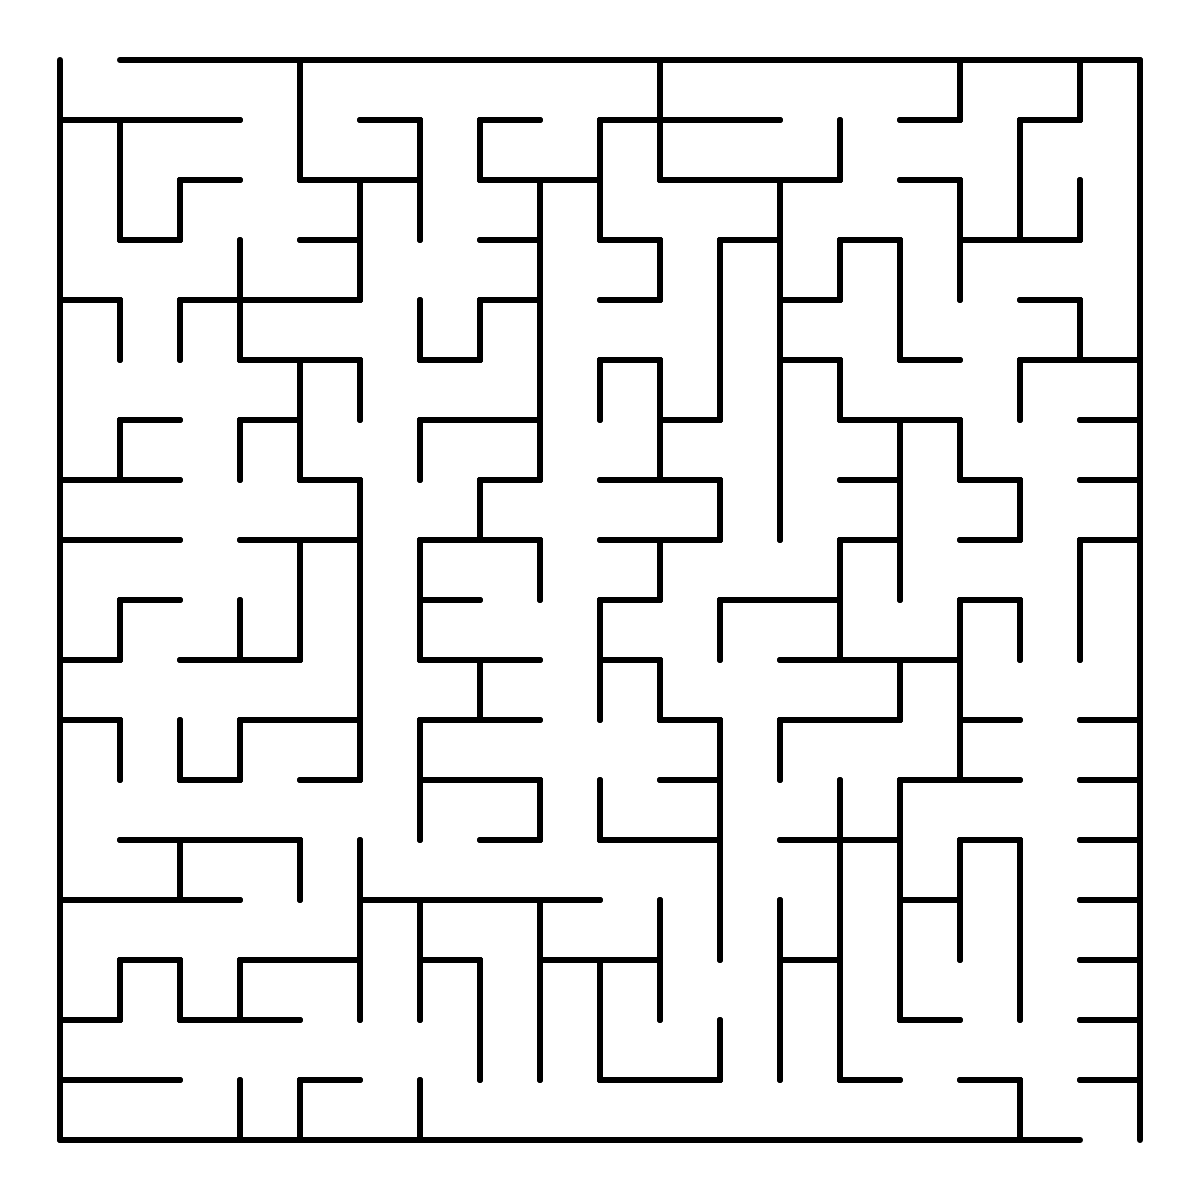
\includegraphics[width=0.27\textwidth]{report/pics/2D_maze.png}%
        \label{fig:a}%
        }%
    \hfill%
    \subfloat[Labyrinthe en 3 dimensions.]{%
        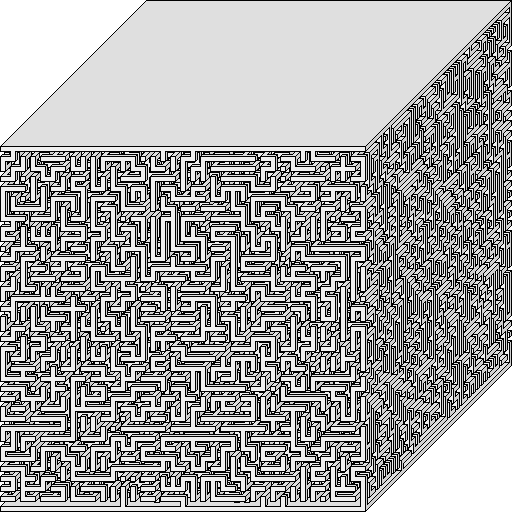
\includegraphics[width=0.27\textwidth]{pics/3D_maze.png}%
        \label{fig:b}%
        }%
    \caption{Exemple d'un labyrinthe 2D et d'un labyrinthe 3D}
\end{figure*}


\subsection{Tessellation d'un labyrinthe}
La classe de tessellation est la géométrie des cellules individuelles qui composent le labyrinthe. Il existe de nombreux types de tessellation, on citera notamment :
\begin{itemize}
\item\textbf{ Tesellation orthogonale :} Il s'agit d'une grille rectangulaire standard où les cellules ont des passages qui se coupent à angle droit formant des cellules sous forme de carrés.

\item\textbf{Tesellation delta :} Un labyrinthe à tessellation delta est un composé de triangles imbriqués, où chaque cellule peut avoir jusqu'à trois passages connectés.

\item\textbf{Tesellation theta :} Un labyrinthe à tessellation theta est composé de cercles concentriques. Les cellules ont généralement quatre connexions de passage possibles, mais peuvent en avoir plus en raison du plus grand nombre de cellules dans les anneaux externes.
\end{itemize}

\begin{figure*}[htp] 
    \centering
    \subfloat[Labyrinthe orthogonal.]{%
        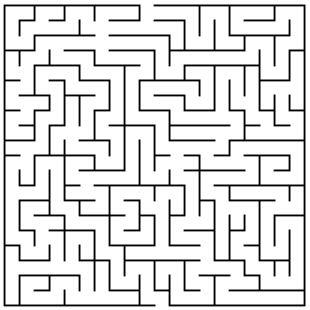
\includegraphics[width=0.27\textwidth]{report/pics/orthogonal_maze.png}%
        \label{fig:a}%
        }%
    \hfill%
    \subfloat[Labyrinthe delta.]{%
        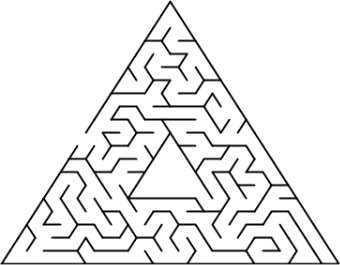
\includegraphics[width=0.3\textwidth]{report/pics/delta_maze.png}%
        \label{fig:b}%
        }%
        \hfill%
    \subfloat[Labyrinthe theta.]{%
        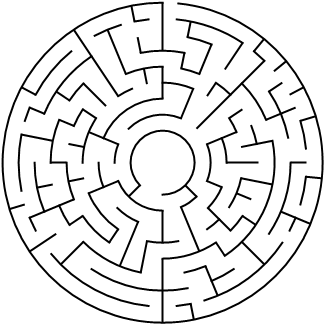
\includegraphics[width=0.3\textwidth]{report/pics/theta_maze.png}%
        \label{fig:c}%
        }%
    \caption{Exemple de labyrinthes avec différentes classes de tessellation.}
\end{figure*}


\subsection{Topologie d'un labyrinthe}
D’un point de vu mathématique, un labyrinthe est définie comme étant une surface connexe pouvant avoir deux types de topologies : topologie simple et topologie comportant des anneaux. Cette différence dans le type de topologie conduit à une distinction des labyrinthes en deux catégories : Les labyrinthes parfaits et les labyrinthes imparfaits.

\subsubsection{Labyrinthe parfait}
Afin qu’un labyrinthe soit labélisé comme étant parfait, ce dernier doit remplir deux conditions :
\begin{itemize}
\item Ne contient pas de cycles.
\item Il existe un unique chemin entre la cellule de départ et la cellule d’arrivée du labyrinthe.
\end{itemize}
Plus généralement, quelque soit deux cellules sélectionnées dans notre labyrinthe, le chemin entre ces deux cellules doit être unique.

\subsubsection{Labyrinthe imparfait}
Un labyrinthe qui ne remplit pas les conditions pour être labélisé comme parfait est dit imparfait. Les labyrinthes imparfaits peuvent donc contenir des boucles, des îlots ou des cellules inaccessibles.


\begin{figure*}[htp] 
    \centering
    \subfloat[Labyrinthe parfait.]{%
        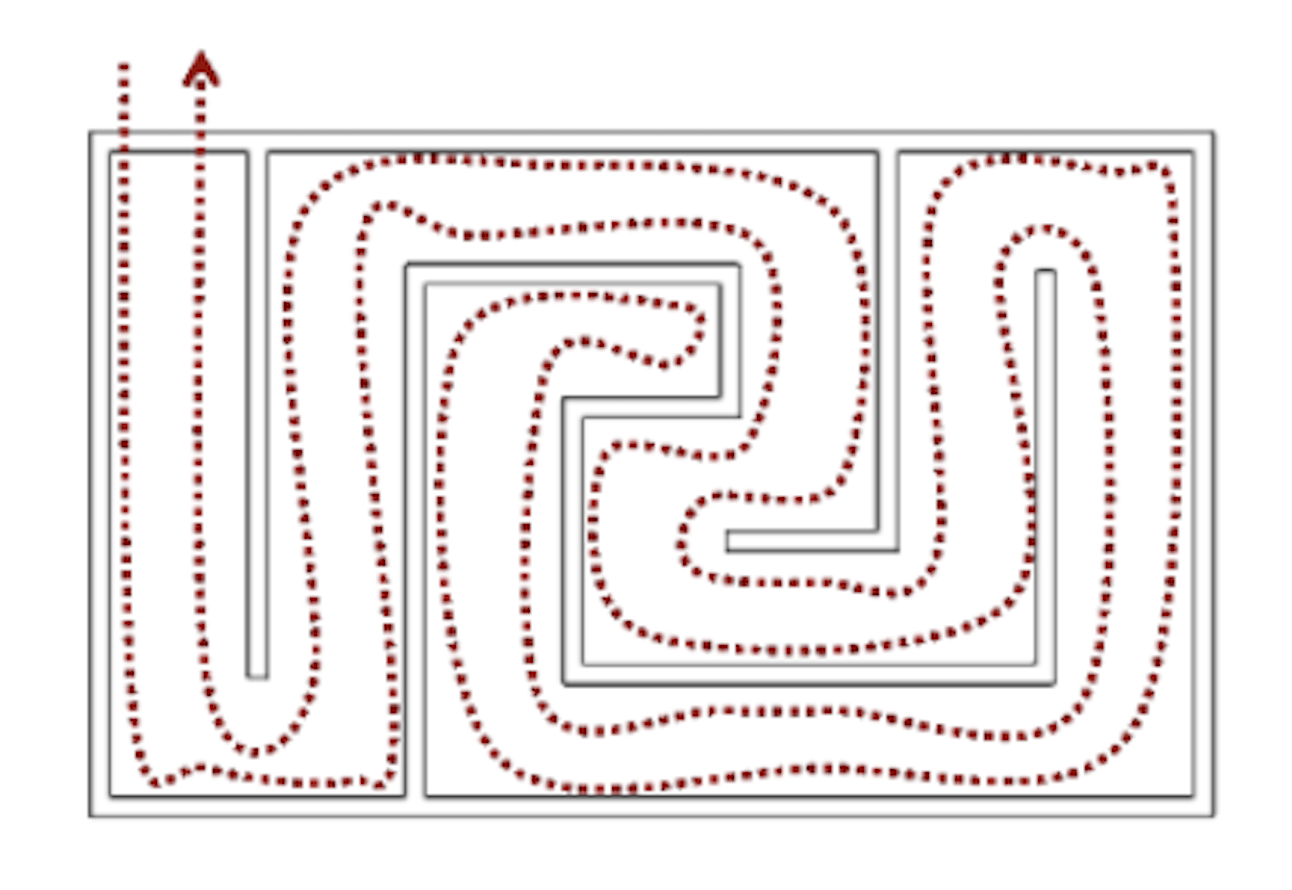
\includegraphics[width=0.5\textwidth]{report/pics/perfect_maze.png}%
        \label{fig:a}%
        }%
    \hfill%
    \subfloat[Labyrinthe imparfait.]{%
        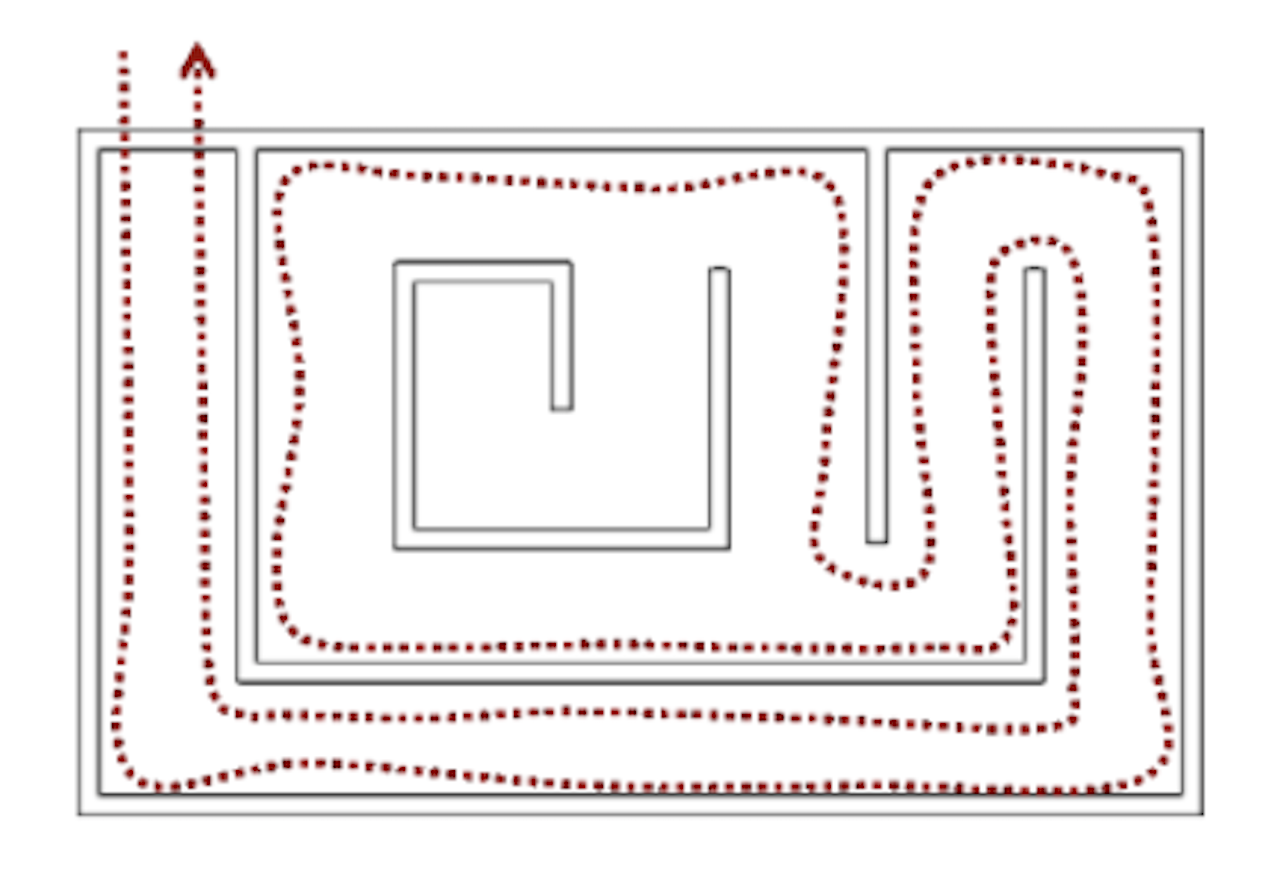
\includegraphics[width=0.5\textwidth]{report/pics/imperfect_maze.png}%
        \label{fig:b}%
        }%
    \caption{Exemple d'un labyrinthe parfait et d'un labyrinthe imparfait.}
\end{figure*}




Dans la suite de ce rapport, nous considérons l'ensemble de nos labyrinthes comme étant de dimension 2 et possédant une tessellation orthogonale. La distinction se feras sur le critère de la topologie, on distinguera alors deux types de labyrinthes : les labyrinthes parfaits et les labyrinthes imparfaits.
\section{Analyse de la problématique de la construction du labyrinthe}
\section{État de l’art: études des solutions existantes} \label{sec:etatDeLart2}

\paragraph{Chapeau}


\section{Solution proposée et sa mise en œuvre} \label{sec:solution2}

\paragraph{Chapeau}


\section{Tests et certifications de la solution} \label{sec:test2}

\paragraph{Chapeau}

\clearpage

\chapter{Partie technique mappage et navigation}
\paragraph{Chapeau du chapitre}
\section{Analyse de la problématique du mappage et navigation du véhicule} \label{sec:Problematiquemappage}

\paragraph{Chapeau}


\section{État de l’art: études des solutions existantes} \label{sec:etatDeLart4}

\paragraph{Chapeau}


\section{Solution proposée et sa mise en œuvre} \label{sec:solution4}

\paragraph{Chapeau}


\section{Tests et certifications de la solution} \label{sec:test4}

\paragraph{Chapeau}

\clearpage

\chapter{Partie technique calcul du plus court chemin}
\paragraph{Chapeau du chapitre}
\section{Analyse de la problématique du plus court chemin} \label{sec:ProblematiquePlusCourtChemin}

\paragraph{Chapeau}


\section{État de l’art: études des solutions existantes} \label{sec:etatDeLart3}

\paragraph{Chapeau}


\section{Solution proposée et sa mise en œuvre} \label{sec:solution3}

\paragraph{Chapeau}


\section{Tests et certifications de la solution} \label{sec:test3}

\paragraph{Chapeau}

\clearpage

\chapter{Partie technique contrôle du véhicule}
\paragraph{Chapeau du chapitre}
\section{Analyse de la problématique du contrôle du véhicule} \label{sec:ProblematiqueControleDuvehicule}

\paragraph{Chapeau}


\section{État de l’art: études des solutions existantes} \label{sec:etatDeLart1}

\paragraph{Chapeau}


\section{Solution proposée et sa mise en œuvre} \label{sec:solution1}

\paragraph{Chapeau}


\section{Tests et certifications de la solution} \label{sec:test1}

\paragraph{Chapeau}

\clearpage

\chapter{Partie technique communication}
\paragraph{Chapeau du chapitre}
\documentclass[10pt]{article}
\usepackage[usenames]{color} %pour la couleur
\usepackage{amssymb} %maths
\usepackage{amsmath} %maths
\usepackage[utf8]{inputenc} %utile pour taper directement les caractères accentués
\begin{document}
\[$
\section{Analyse de la problématique de la communication} \label{sec:ProblematiqueCommunication}
\paragraph{}Puisque nous avons présenté lors des parties précédentes les différentes composantes du projet, il s'agit maintenant de les faire communiquer entre eux. Nous nous interrogerons donc, au cours de cette partie, sur un moyen de communication inter-process entre la simulation en Java/Processing et le brain en C en local (sur une même machine) puis à distance (entre la micromouse et l'IHM).

\section{État de l’art: études des solutions existantes} \label{sec:etatDeLart5}
\paragraph{Pour faire communiquer plusieurs processus, de nombreux moyens existent. Cette partie a pour but d'étudier ces différentes alternatives afin d'en tirer les plus avantageux en fonction de nos besoins.}

  % Sockets - Pipes - Nammed pipes
  \subsection{Communication par sockets}
  \paragraph{}Un socket permet une abstraction de la couche logicielle d'un programme se rapportant au réseau. Il s'appuie sur les modules du système d'exploitation afin de faire communiquer deux processus selon deux modes de connexions :
  \begin{itemize}
    \item le mode connecté s'appuyant sur le protocole de la couche transport TCP (Transmission Control Protocol) qui établit une connexion durable entre les deux interlocuteurs. Ce mode de communication est reconnu comme fiable puisqu'il s'appuie sur un mécanisme d'acquittement et de contrôle CRC (Cyclic Redundancy Control) pour chaque paquet IP envoyé. Une erreur détectée par un de ces deux mécanisme déclenche le renvoi des données alors perdues ou corrompues ;
    \item le mode non-connecté utilisant le protocole de la couche transport UDP (User Datagram Protocol) qui présente l'avantage d'être plus léger puisqu'il s'affranchit des mécanismes d'acquittement et de contrôle cités précédemment.
  \end{itemize}

  \paragraph{}Ainsi, si dans notre projet, sockets il y a, c'est le mode non-connecté qui sera privilégié. En effet, les données échangées étant soumises à des contraintes de temps réels, lorsqu'un paquet IP est perdu, il n'est pas utile de le renvoyer car les données qu'il porte sont alors inactuelles et donc inutilisables.

  \paragraph{}Dans le langage C, ces deux types sockets sont implémentés dans la bibliothèque \texttt{<sys/socket.h>} alors qu'en Java/Processing, c'est la bibliothèque \texttt{hypermedia.net.*} qui est utilisée pour la création de socket UDP.

  \fig{pics/udp_socket.png}{15cm}{12cm}{Diagramme décrivant le fonctionnement des sockets UDP}{udp_socket}

  \paragraph{}Par ailleurs, la communication par sockets adopte une architecture clients/serveur. Il est donc possible d'envisager un dispositif composé de plusieurs micromouses en utilisant cette solution de communication ; la partie simulation représentant le serveur et les brains, les clients.


\section{Solution proposée et sa mise en œuvre} \label{sec:solution5}
\paragraph{Au vu des choix matériels, nous avons opté pour les canaux nommés afin de faire communiquer les différentes composantes du projet. En effet, notre micromouse ne possédant pas de carte réseau, c'est par Bluetooth que se fera le communication entre les deux programmes. Ainsi, bien qu'elle semblait être la plus adaptée, la solution employant les sockets se retoruve alors inutilisable dans le contexte décrit.}

  \subsection{Qu'est-ce qu'un canal nommé (named pipe) ?}
  \paragraph{}



\section{Tests et certifications de la solution} \label{sec:test5}
\paragraph{Chapeau}
$\]
\end{document}
\clearpage

\chapter{Rendu final}
\paragraph{Chapeau du chapitre}
\section{Interface utilisateur finale}
\label{sec:rendu_final_interface_utilisateur_finale}

\paragraph{Chapeau}


\section{Tests utilisateur et certification}
\label{sec:rendu_final_tests_utilisateur_et_certification}

\paragraph{Chapeau}


\section{Autres tests et certifications}
\label{sec:rendu_final_autres_tests_et_certifications}

\paragraph{Chapeau}
\clearpage

\chapter{Gestion de projet}
\paragraph{Chapeau du chapitre}
\section{Méthode de gestion} \label{sec:methodeGestion}

\paragraph{Chapeau}


\section{Répartition de tâches} \label{sec:repartTaches}

\paragraph{Chapeau}


\section{Choix n°1} \label{sec:gestionC1}

\paragraph{Chapeau}


\section{Choix n°2} \label{sec:gestionC2}

\paragraph{Chapeau}

\clearpage

\chapter{Conclusion et perspectives}
\paragraph{Chapeau du chapitre}
\section*{Conclusion} \label{sec:conclusion}

\paragraph{Chapeau}


\section*{Perspectives} \label{sec:perspectives}

\paragraph{Chapeau}

\clearpage

\bibliographystyle{plain}
\bibliography{bibliographies}
\clearpage

\section*{Annexe}
\label{sec:annexe}

\paragraph{Chapeau}
\clearpage

\end{document}
